\section{Experiments}
\label{sec:experiments}

\subsection{Experimental Setup}
\label{sec:setup}

\paragraph{Models.}
We probe three instruction-tuned models with comparable parameter counts but distinct architectures: Llama-3.1-8B-Instruct (32 layers, hidden dimension 4096) \citep{grattafiori2024llama}, Qwen3-8B (36 layers, hidden dimension 4096) \citep{yang2025qwen3}, and Gemma-2-9B-IT (42 layers, hidden dimension 3584) \citep{team2024gemma}.
The three models were independently verified on ConflictQA \citep{xie2024adaptive}, yielding only 3.5\% three-way question overlap (23 questions); pairwise overlaps range from 7.2\% (Llama $\cap$ Gemma) to 24.8\% (Gemma $\cap$ Qwen), so the consistent asymmetry pattern constitutes largely independent replication.

\paragraph{Dataset and translation.}
After parametric knowledge verification (\S\ref{sec:data}), we retain 1{,}368 samples for Llama (1{,}096 train / 272 test), 966 for Qwen (773 / 193), and 1{,}590 for Gemma (1{,}274 / 316), split 80/20 with stratification.
All inputs are translated into Chinese using COMET-validated translations (\S\ref{sec:data}).

\paragraph{Probing.}
For each layer, we train an $L_2$-regularized logistic regression probe on the last-token residual stream (\S\ref{sec:extraction}).
We report balanced accuracy rather than AUROC, as our claims depend on cross-model directional comparisons; AUROC results are in Appendix~\ref{app:auroc}.
All CIs are computed via bootstrap resampling with paired differences for asymmetry estimation.
A selectivity control \citep{hewitt2019designing} with permuted labels on matched-condition data ($N{=}131$--$201$) yields near-chance accuracy (49.2--51.0\%) across all models, confirming selectivity gaps of 21--40~pp.
All experiments used a single GPU; the boundary replication (Appendix~\ref{app:boundary}) used an NVIDIA RTX PRO 6000.

\paragraph{Non-conflict baseline.}
To test whether cross-lingual transfer patterns are specific to knowledge conflicts, we run the same probing pipeline on XNLI \citep{conneau2018xnli}, classifying entailment versus contradiction (\S\ref{sec:confound_method}).

\subsection{Within-Language Conflict Detection}
\label{sec:within_lang}

Table~\ref{tab:main_results} reports balanced accuracy for all probe transfer directions.
All three models encode linearly detectable conflict signals in their residual streams.
Llama achieves 77.6\% on EN$\to$EN (peak at layer 15, 47\% depth) and 72.1\% on ZH$\to$ZH.
Qwen reaches 75.0\% on EN$\to$EN (peak at layer 24, 67\% depth) and 72.6\% on ZH$\to$ZH.
Gemma attains 76.2\% on EN$\to$EN (peak at layer 24, 57\% depth) and 71.0\% on ZH$\to$ZH.
All within-language accuracies are significantly above chance (binomial $p < 0.001$).
Figure~\ref{fig:layer_probe} shows the layer-wise probe accuracy curves for all three models.
These results confirm that knowledge conflict signals are linearly separable in the residual stream across all three architectures and both languages.

%% Figure 2: Layer-wise probe accuracy
\begin{figure*}[t]
\centering
\vspace{-5pt}
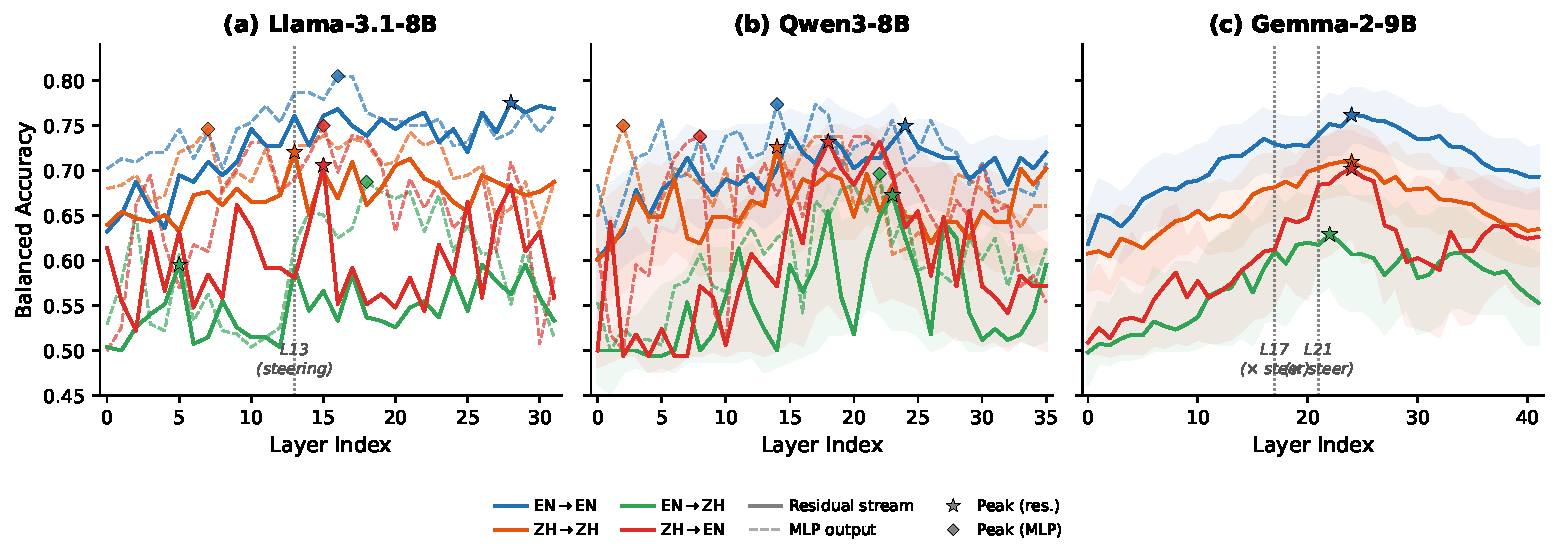
\includegraphics[width=0.92\textwidth]{fig2_layerwise_probes.pdf}
\vspace{-8pt}
\caption{Layer-wise probe balanced accuracy for Llama-3.1-8B (left), Qwen3-8B (center), and Gemma-2-9B-IT (right). Solid lines: residual stream probes; dashed lines (Llama and Qwen only): multilayer perceptron (MLP) sublayer probes. Stars mark peak layers. In the Llama panel, the vertical annotation at L13 marks the layer where steering produces significant causal influence (Fisher $p < 0.001$), near the EN$\to$EN probe peak (L15). In the Gemma panel, L17 and L21 are annotated as steering-negative layers.}
\label{fig:layer_probe}
\vspace{-10pt}
\end{figure*}

\subsection{Cross-Lingual Transfer and Asymmetry}
\label{sec:cross_lingual}

All four cross-lingual transfer directions achieve balanced accuracy above chance (binomial $p < 0.001$; Table~\ref{tab:main_results}); this confirms that conflict representations partially overlap between English and Chinese.
All three models show a consistent directional trend: probes trained on Chinese representations transfer to English (ZH$\to$EN) more accurately than the reverse direction (EN$\to$ZH).
We define $\Delta_{\text{asym}} = \text{acc}(\text{ZH}{\to}\text{EN}) - \text{acc}(\text{EN}{\to}\text{ZH})$, computed via paired bootstrap.
For Llama, $\Delta_{\text{asym}} = +7.3$ percentage points (pp) with a 95\% bootstrap CI of [0.4, 14.0] ($p = 0.038$); for Qwen, $\Delta_{\text{asym}} = +7.2$ pp with CI [$-$0.6, 13.7]; for Gemma, $\Delta_{\text{asym}} = +6.6$ pp with CI [1.9, 11.1] ($p = 0.006$).
While the Qwen CI marginally includes zero, the asymmetry is consistent in direction across all three architectures.
The magnitude of this asymmetry is consistent in direction and magnitude with the XNLI non-conflict baseline across all three architectures (\S\ref{sec:xnli_baseline}), and the consistent direction across all three models suggests a shared structural property rather than a model-specific artifact (Figure~\ref{fig:asymmetry_forest}).

\begin{table}[t]
\centering
\caption{Single-seed balanced accuracy (\%) at each direction's optimal layer. $\Delta_{\text{asym}}$ and 95\% CIs from paired bootstrap ($n = 2{,}000$ resamples). Bold: best per-task direction.}
\label{tab:main_results}
\small
\resizebox{\columnwidth}{!}{%
\begin{tabular}{lccc}
\toprule
Direction & Llama-3.1-8B & Qwen3-8B & Gemma-2-9B \\
\midrule
\multicolumn{4}{l}{\textit{Conflict Task}} \\
EN $\to$ EN & \textbf{77.6} & \textbf{75.0} & \textbf{76.2} \\
ZH $\to$ ZH & 72.1 & 72.6 & 71.0 \\
EN $\to$ ZH & 59.6 & 67.3 & 62.9 \\
ZH $\to$ EN & 70.6 & 73.2 & 70.2 \\
$\Delta_{\text{asym}}$ & +7.3 [0.4, 14.0] & +7.2 [$-$0.6, 13.7] & +6.6 [1.9, 11.1] \\
\midrule
\multicolumn{4}{l}{\textit{XNLI Baseline}} \\
EN $\to$ EN & 94.0 & 96.6 & 95.6 \\
ZH $\to$ ZH & 87.5 & 89.5 & 89.0 \\
EN $\to$ ZH & 89.0 & 90.5 & 89.4 \\
ZH $\to$ EN & \textbf{94.9} & \textbf{97.2} & \textbf{97.5} \\
$\Delta_{\text{asym}}$ & +6.0 [0.9, 11.3] & +6.7 [2.4, 11.7] & +7.8 [5.7, 10.0] \\
\bottomrule
\end{tabular}%
}
\begin{flushleft}
\footnotesize Note: $\Delta_{\text{asym}}$ is the mean of paired bootstrap differences, not the arithmetic difference of the reported single-seed accuracies.
\end{flushleft}
\end{table}

\subsection{Non-Conflict Baseline Comparison}
\label{sec:xnli_baseline}

If the ZH$\to$EN transfer advantage were conflict-specific, it should be absent in a non-conflict task.
XNLI entailment-versus-contradiction probes exhibit the same directional asymmetry: Llama $\Delta_{\text{asym}} = +6.0$~pp, CI [0.9, 11.3]; Qwen $+6.7$~pp, CI [2.4, 11.7]; Gemma $+7.8$~pp, CI [5.7, 10.0] ($p < 0.001$).
All XNLI CIs exclude zero and overlap with the conflict-task CIs (Figure~\ref{fig:asymmetry_forest}).
TOST (Two One-Sided Tests) equivalence tests ($\pm$2~pp margin) are non-significant ($p > 0.36$, power $= 1.4\%$), reflecting insufficient power rather than meaningful differences; the consistent direction across all six model$\times$task combinations (binomial $p = 0.016$) and magnitudes clustering in [$+$6.0, $+$7.8~pp] support the consistency characterization.

%% Figure 3: Asymmetry forest plot
\begin{figure}[t]
\centering
\vspace{-5pt}
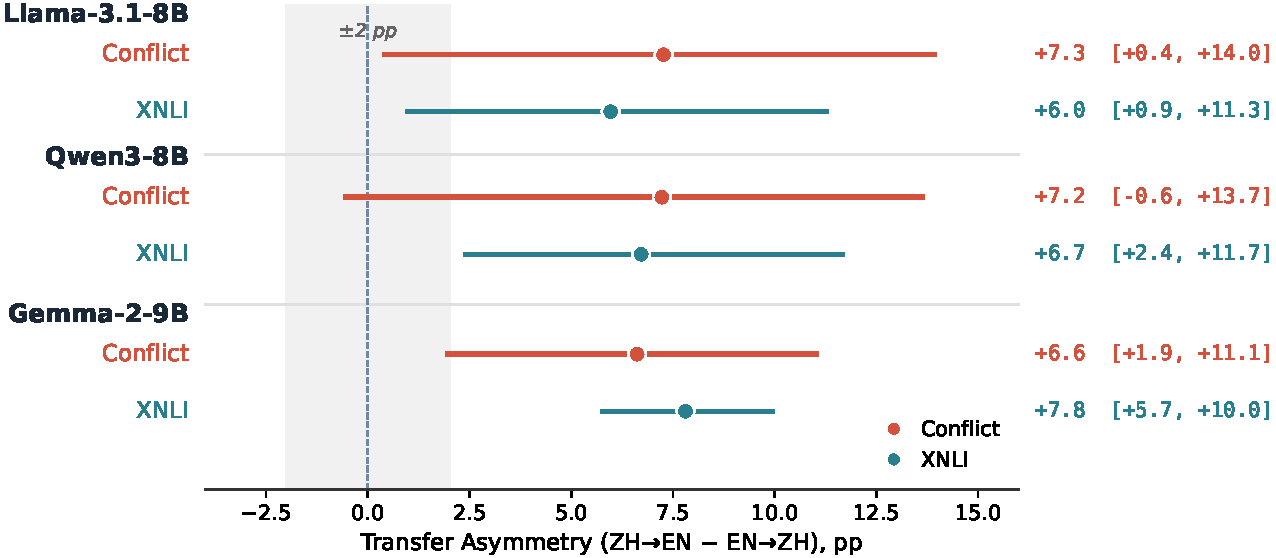
\includegraphics[width=\columnwidth]{fig4_asymmetry_forest.pdf}
\vspace{-8pt}
\caption{Transfer asymmetry ($\Delta_{\text{asym}}$) with bootstrap 95\% CIs ($n = 2{,}000$) for conflict and XNLI tasks across all three architectures (six data points). Conflict and XNLI CIs overlap substantially within each model, indicating that the ZH$\to$EN advantage is a general cross-lingual property rather than conflict-specific. Grey dashed lines: $\pm$2~pp exploratory equivalence margin (TOST power $= 1.4$\%; see \S\ref{sec:xnli_baseline}).}
\label{fig:asymmetry_forest}
\vspace{-10pt}
\end{figure}

\subsection{Confound Exclusion}
\label{sec:confounds}

Two potential confounds could inflate cross-lingual probe accuracy: lexical overlap between English and Chinese inputs and translation quality.

\paragraph{Token overlap and EN-DE control.}
Per-sample Jaccard similarity between English and Chinese tokenized inputs averages 3--4\%, already at the floor imposed by distinct writing systems.
Neither model shows a positive correlation between token overlap and probe accuracy: Qwen yields no significant correlation ($p > 0.4$), and Llama shows a weak negative correlation ($r = -0.15$, $p = 0.012$, $r^2 = 0.023$), running counter to the confound hypothesis.
The strongest evidence comes from a typological control: we translate the same Llama ConflictQA samples into German using the identical Qwen3-8B pipeline, where per-sample Jaccard similarity (14.8\%) is approximately $4\times$ higher than EN-ZH (3.8\%).
Despite this substantially higher lexical overlap, the EN$\leftrightarrow$DE transfer asymmetry is near-zero ($\Delta = +1.2$~pp, n.s.), ruling out shared tokens as a driver of the observed EN-ZH asymmetry (Table~\ref{tab:confound}).

\paragraph{Translation quality.}
We stratify test samples by COMET score into terciles and compare EN$\to$ZH probe accuracy across strata.
Qwen shows a reversed association ($\Delta = -5.6$~pp, Fisher $p = 0.695$) and Llama a negligible one ($\Delta = +1.7$~pp, $p = 0.761$), both inconsistent with translation quality driving probe transfer.
Gemma shows a non-significant trend in the confound direction ($\Delta = +10.3$~pp, $p = 0.278$), but interpretation is limited by the near-chance baseline accuracy of the EN$\to$ZH probe at L17 (58.8\%), placing this analysis in a low-power regime.
With a minimum detectable difference of 25.3~pp at 80\% power ($n \approx 56$ per tercile), the COMET tercile analysis can neither confirm nor exclude a moderate translation quality effect; it serves as supplementary evidence alongside the token overlap and EN-DE controls.

\begin{table}[t]
\centering
\caption{Confound exclusion analysis. COMET tercile: $\Delta$ = balanced accuracy difference between high and low COMET score terciles for EN$\to$ZH probes (Fisher's exact test). Token overlap: Pearson correlation between per-sample Jaccard similarity and EN$\to$ZH probe accuracy.}
\label{tab:confound}
\resizebox{\columnwidth}{!}{%
\begin{tabular}{llrl}
\toprule
Confound & Model & Result & $p$ \\
\midrule
COMET tercile & Qwen & $\Delta = -5.6$ pp & 0.695 \\
COMET tercile & Llama & $\Delta = +1.7$ pp & 0.761 \\
COMET tercile & Gemma & $\Delta = +10.3$ pp & 0.278 \\
\midrule
Token overlap & Qwen & n.s. & $>$0.4 \\
Token overlap & Llama & $r = -0.15$ & 0.012 \\
\bottomrule
\end{tabular}%
}
\end{table}

\subsection{Causal Evidence via Representation Steering}
\label{sec:steering}

The probing results establish that conflict signals are detectable, but detection does not imply causal relevance.
We test whether the probe weight direction $\mathbf{w}_l$ causally influences conflict resolution by injecting $\alpha \cdot \mathbf{w}_l$ into the last-token residual stream at a target layer during inference.
We sweep $\alpha \in \{\pm 20, \pm 10, \pm 5, \pm 2, \pm 1\}$ ($k = 10$) following prior steering conventions \citep{turner2023activation, marks2024geometry} and report results at all tested values.
We measure the flip rate (fraction of samples that switch answer category) and compare against a random-direction control of equal magnitude via Fisher's exact test.

\paragraph{L13 (mid-layer, 41\% depth).}
Steering at layer 13 produces bidirectional causal effects (Figure~\ref{fig:steering_viz}; Table~\ref{tab:steering}):
Positive steering ($\alpha = +5$) yields a flip rate of 19.9\% versus 6.6\% for the random control (Fisher $p = 0.002$; 4 parametric-to-contextual [p$\to$c] flips), while negative steering ($\alpha = -20$) yields 36.0\% versus 17.6\% ($p < 0.001$; 5 contextual-to-parametric [c$\to$p] flips); both survive per-layer Bonferroni correction ($k{=}10$, threshold $p < 0.005$).
All-position injection at L13 produces identical results; the causal signal is concentrated at the final token.
Steering at nearby L16 (50\% depth, just three layers away) showed no significant effect (all $p > 0.12$), consistent with a narrow causal window.
Under a conservative family-wise correction across all 30 tests (3 layers $\times$ 10 $\alpha$ values, threshold $p < 0.00167$), L13 remains significant ($\alpha = -20$, $p < 0.001$).
An independent replication ($N = 201$, six layers L12--L28; Appendix Table~\ref{tab:boundary}) confirmed L13 significance ($p < 0.001$) and localized the causal boundary: effects attenuate from L14 ($p = 0.002$) through L16 ($p = 0.005$) to non-significance at L18 ($p = 0.010$, n.s.\ after Bonferroni) and L28 ($p = 0.284$).

\begin{figure*}[t]
\centering
\vspace{-5pt}
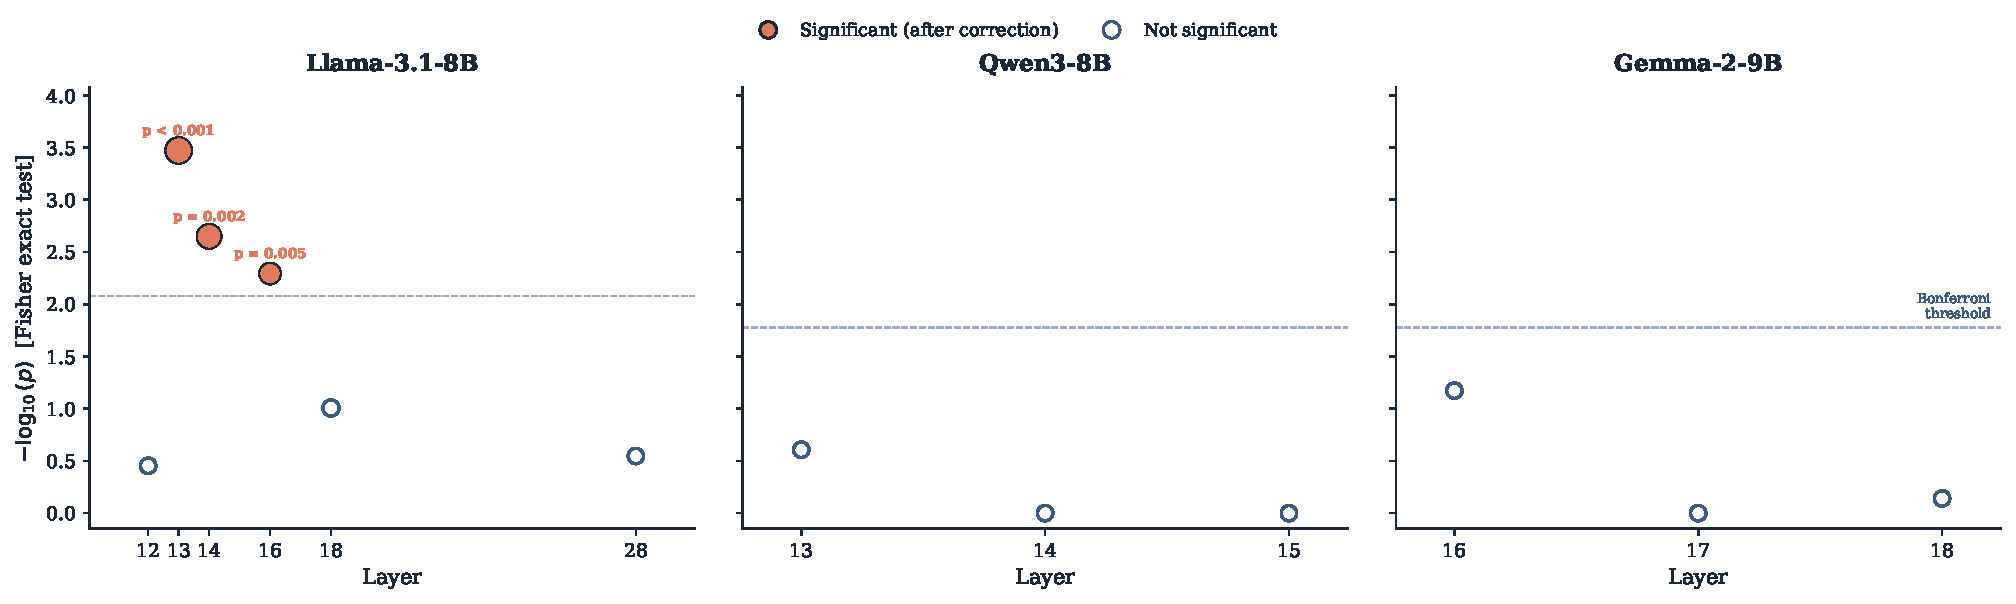
\includegraphics[width=\textwidth]{fig5_steering.pdf}
\vspace{-8pt}
\caption{Steering significance across layers and models. Each point shows the best $-\log_{10}(p)$ (Fisher exact test) across six $\alpha$ values at a given layer. Filled circles: significant after per-layer Bonferroni correction ($k{=}6$, threshold $p < 0.0083$). Only Llama shows significant causal effects, concentrated at L13 ($p < 0.001$) with attenuation through L14 ($p = 0.002$) and L16 ($p = 0.005$). Qwen (L13--L15) and Gemma (L16--L18) show no significant effects at comparable relative depths (36--43\%), despite high probe accuracy.}
\label{fig:steering_viz}
\vspace{-14pt}
\end{figure*}

\paragraph{Negative layers and coherence collapse.}
Steering at L28 (88\% depth) produces no significant effect with either last-token or all-position injection (all $p > 0.3$); L18 (MLP peak, 56\%) is similarly negative ($p > 0.44$).
At extreme magnitude ($\alpha = +20$), the control flip rate exceeds steering ($p = 0.053$), indicating coherence collapse.

\paragraph{Causal localization (Llama).}
Causal influence is localized to L13 (41\% depth), near but distinct from the probe peak (L15, 47\%): upper layers retain detectable signal but lack causal influence.
An independent replication (seed=123, different split) confirms L13: 2/6 $\alpha$ values survive Bonferroni ($p < 0.0083$), matching the original (Appendix~\ref{app:seed_replication}).

\paragraph{Cross-model steering.}
Cross-model experiments use the reduced 6-value $\alpha$ grid ($k{=}6$, per-layer threshold $p < 0.0083$; \S\ref{sec:steering_method}).
Qwen L14 (39\%, $n = 131$) produced no significant effect (best $p = 0.785$) and zero flips.
Gemma L17 (40\%, $n = 171$) provides a stronger test: with 88.9\% probe accuracy (the highest among all models), steering produced no significant change (best $p = 0.448$) and zero flips, ruling out probe quality as a confound.
AUROC analysis confirms: Gemma achieves 0.93 AUROC (vs.\ Llama 0.98, Qwen 0.77; Appendix~\ref{app:auroc}), yet steering produces zero causal effect.
Matched-condition results at ${\sim}$36--43\% depth across all models confirm the null (Appendix~\ref{app:steering_config}).

\begin{table}[t]
\centering
\caption{Representation steering results (Llama: original experiment, $N{=}136$, 10-value $\alpha$ grid; Qwen/Gemma: 6-value grid). Flip rate: fraction of test samples switching answer category. Control: random-direction perturbation of equal magnitude. Bonferroni threshold $p < 0.005$ ($k = 10$) for Llama, $p < 0.0083$ ($k = 6$) for Qwen/Gemma. Significant results in bold.$^{\dagger}$}
\label{tab:steering}
\small
\resizebox{\columnwidth}{!}{%
\begin{tabular}{lcrrrrl}
\toprule
Layer & Depth & $\alpha$ & Steer (\%) & Ctrl (\%) & Fisher $p$ & Dir. \\
\midrule
\textbf{L13} & \textbf{41\%} & $\mathbf{+5}$ & \textbf{19.9} & \textbf{6.6} & $\mathbf{0.002}$ & \textbf{4 p$\to$c} \\
\textbf{L13} & \textbf{41\%} & $\mathbf{-20}$ & \textbf{36.0} & \textbf{17.6} & $\mathbf{<0.001}$ & \textbf{5 c$\to$p} \\
L16 & 50\% & $+5$ & 8.8 & 8.1 & 1.000 & \\
L16$^{\S}$ & 50\% & $+10$ & 18.4 & 11.0 & 0.123 & \\
L16 & 50\% & $+20$ & 22.8 & 24.3 & 0.886 & \\
L18 & 56\% & $+2$ & 3.7 & 1.5 & 0.447 & \\
L28 & 88\% & $-20$ & 14.7 & 16.9 & 0.740 & \\
L28 (all) & 88\% & $-20$ & 11.8 & 11.8 & 1.000 & \\
\midrule
\multicolumn{7}{l}{\textit{Qwen3-8B ($n_{\text{test}} = 131$)}} \\
L14 & 39\% & best & \multicolumn{2}{c}{n.s.} & 0.785 & 0 dir. \\
\midrule
\multicolumn{7}{l}{\textit{Gemma-2-9B-IT ($n_{\text{test}} = 171$)$^{\ddagger}$}} \\
L17 & 40\% & best & \multicolumn{2}{c}{n.s.} & 0.448 & 0 dir. \\
\bottomrule
\end{tabular}%
}
\begin{flushleft}
\footnotesize $^{\dagger}$ At $\alpha = +20$, the control flip rate exceeds steering ($p = 0.053$), indicating coherence collapse at extreme perturbation magnitudes. $^{\ddagger}$ Gemma: after correcting a label assignment error. $^{\S}$ L16 original ($N{=}136$); replication ($N{=}201$) yields $p = 0.005$ (\S\ref{sec:steering}).
\end{flushleft}
\vspace{-8pt}
\end{table}